% Koko
\documentclass[ichigo,normal,cn]{elegantnote_mod}
\usepackage{tikz}
\usetikzlibrary{shapes,snakes}
\newfontfamily\courier{Courier New}
\lstset{linewidth=1.1\textwidth,
	numbers=left,
	basicstyle=\small\courier,
	numberstyle=\tiny\courier,
	keywordstyle=\color{blue}\courier,
	commentstyle=\it\color[cmyk]{1,0,1,0}\courier, 
	stringstyle=\it\color[RGB]{128,0,0}\courier,
	frame=single,
	backgroundcolor=\color[RGB]{245,245,244},
	breaklines,
	extendedchars=false, 
	xleftmargin=2em,xrightmargin=2em, aboveskip=1em,
	tabsize=4, 
	showspaces=false
	basicstyle=\small\courier
}
\title{Vivado 设计流程}

\begin{document}
\maketitle

Vivado 有两种开发模式,Project Mode 和 Non-Project Mode。
两者的主要区别是,Project Mode 使用 Flow Navigation 更加自动化,
Non-Project Mode 使用 Tcl 命令直接控制操作,更手动但更不受限制。
实际中根据开发需求选择这两种模式,一般简单设计中采用 Project Mode。

下面我们将通过以流水灯实验为例了解如何使用 Xilinx Vivado
进行最基本的 FPGA 设计。

\section{使用 Vivado 进行 FPGA 设计的一般流程}

在介绍 Vivado 工具的使用前,先简单介绍下数字电路设计的一般流程,
如图~\ref{fig:STAFlow}~ 所示,图中的最后步骤 ``Sign off'' 为物理签核,
也就是得到最终的电路版图。将电路版图交付晶元代工厂,就可以生产芯片了。 

\begin{figure}[!htbp]
    \centering
    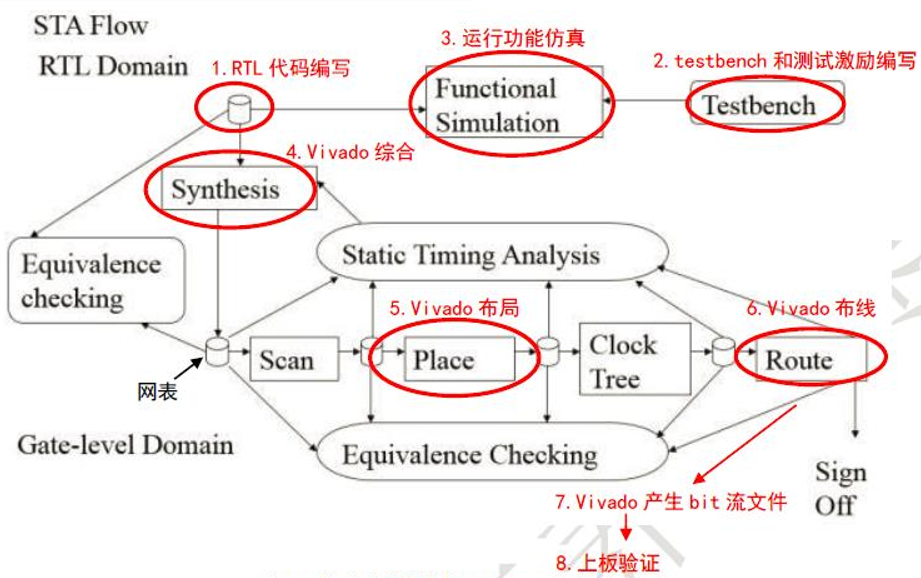
\includegraphics[width=.8\textwidth]{fig/STAFlow}
    \caption{数字设计的一般流程 \textbf{Source: 龙芯}}
    \label{fig:STAFlow}
\end{figure}

FPGA 的开发流程可以看作是一般数字电路设计流程的简化版本,其核心步骤是
与一般数字设计流程一一对应的,图中的红色部分就是 FPGA 的开发流程。在 FPGA
开发的最后一步是生成 bit 文件并下载到 FPGA 中进行运行,而不是通常电路开发的
生成电路版图。

\section{新建 Vivado 工程}

通过双击桌面上的 “Vivado 2019.1” 快捷方式,或是在开始菜单的 “Xilinx Design Tools”
文件夹内找到对应的程序并单击以后。等待一会就会出现 Vivado 的主界面。单击主界面的 “Quick Start”
选项卡下的 “Create Project” 即可打开新建工程向导开始创建项目。

\begin{figure}[!htbp]
    \centering
    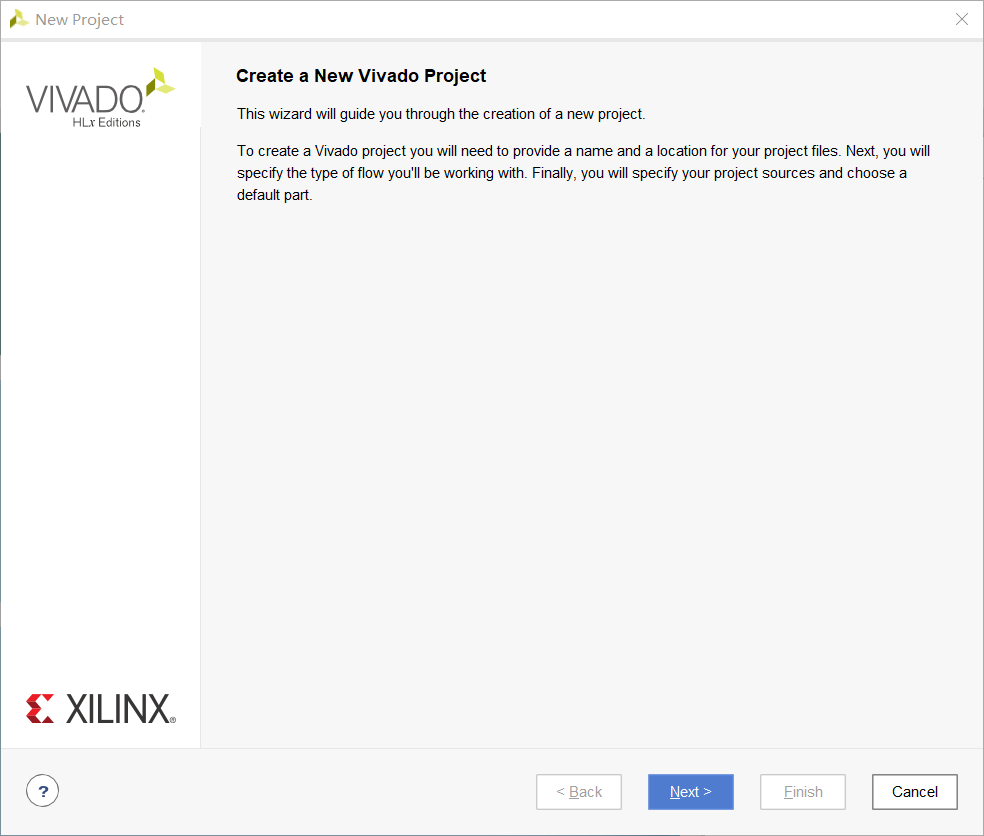
\includegraphics[width=.8\textwidth]{fig/Create1}
    \caption{新建工程向导}
    \label{fig:Create1}
\end{figure}

点击 ``Next'',进入图~\ref{fig:Create2}~ 所示界面。

\begin{figure}[!htbp]
    \centering
    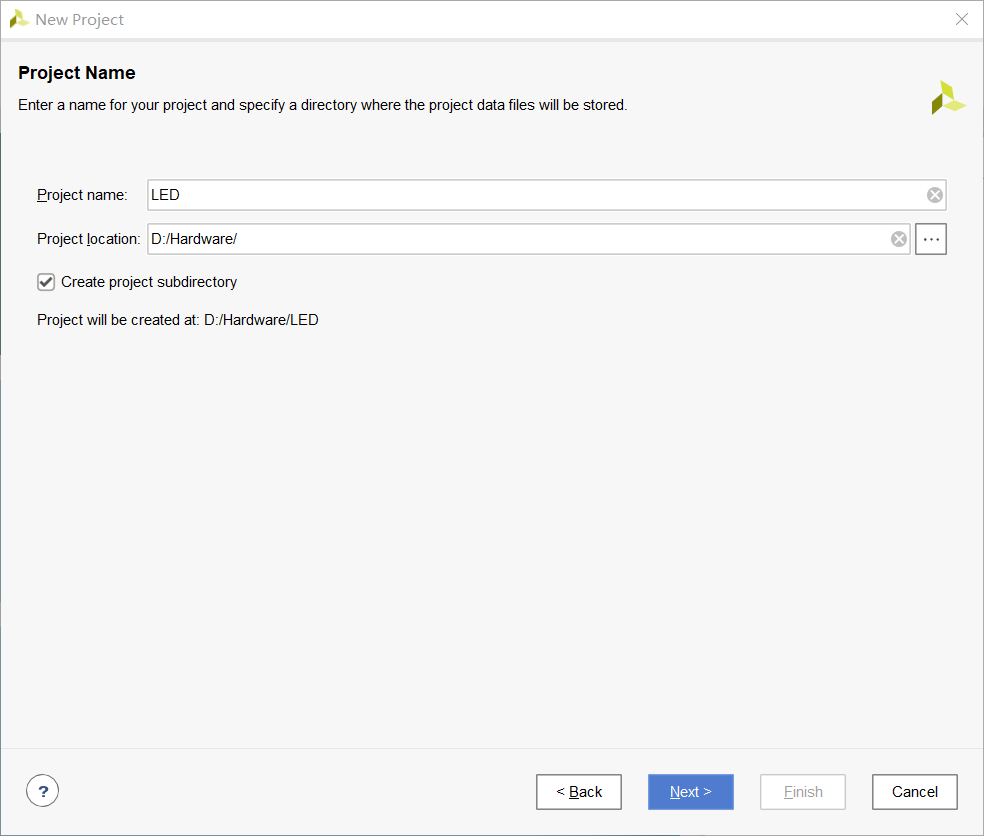
\includegraphics[width=.8\textwidth]{fig/Create2}
    \caption{设置项目名称、地址}
    \label{fig:Create2}
\end{figure}

输入工程名称并选择工程的文件位置,并勾选 ``Create project subdirectory'' 选项,
为工程在指定存储路径下建立独立的文件夹。设置完成后,点击 ``Next'',进入图~\ref{fig:Create3}~ 所示界面。

\tikzstyle{mybox} = [draw=red, fill=blue!5, very thick,
    rectangle, rounded corners, inner sep=10pt, inner ysep=15pt]
\tikzstyle{fancytitle} =[fill=red, text=white]

\tikzstyle{normalbox} = [draw=black!80, fill=blue!5, very thick,
    rectangle, rounded corners, inner sep=10pt, inner ysep=15pt]
\tikzstyle{normaltitle} =[fill=black!80, text=white]

\begin{center}
    \begin{tikzpicture}
        \node [mybox] (box){%
            \begin{minipage}{0.9\textwidth}
                \qquad 工程名称和存储路径中\textbf{不能}出现中文和空格,
                建议工程名称以字母、数字、下划线来组成。 
            \end{minipage}
        };
        \node[fancytitle, right=10pt] at (box.north west) {注意};
    \end{tikzpicture}
\end{center}

选择 “RTL Project” 一项,并勾选 “Do not specify sources at this time”,
勾选该选项是为了跳过在新建工程的过程中添加设计源文件,
如果你需要在新建工程时添加源文件的话则无需勾选。点击 “Next”,进入图~\ref{fig:Create4}~ 所示界面。

\begin{figure}[!htbp]
    \centering
    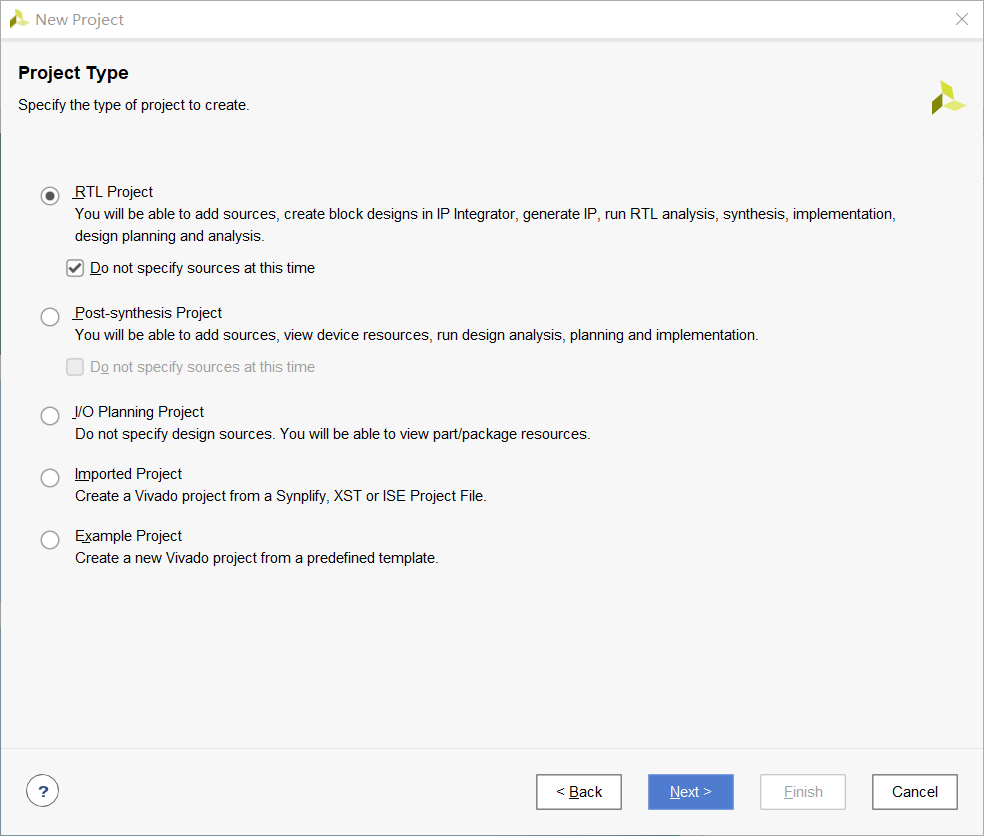
\includegraphics[width=.8\textwidth]{fig/Create3}
    \caption{设置工程类型}
    \label{fig:Create3}
\end{figure}

根据使用的 FPGA 开发平台,选择对应的 FPGA 目标器件。
根据实验平台搭载的 FPGA,在筛选器的 “Family” 选择 “Artix 7”,
在筛选得到的型号里面选择 “\textbf{\textcolor{ichigo}{xc7a35tcsg324-1}}”。点击 “Next”,
向导会列出项目信息,确认信息一致无误后,点击 “Finish” 完成项目的建立,如果信息有误
可以返回重新设置。 

\begin{figure}[!htbp]
    \centering
    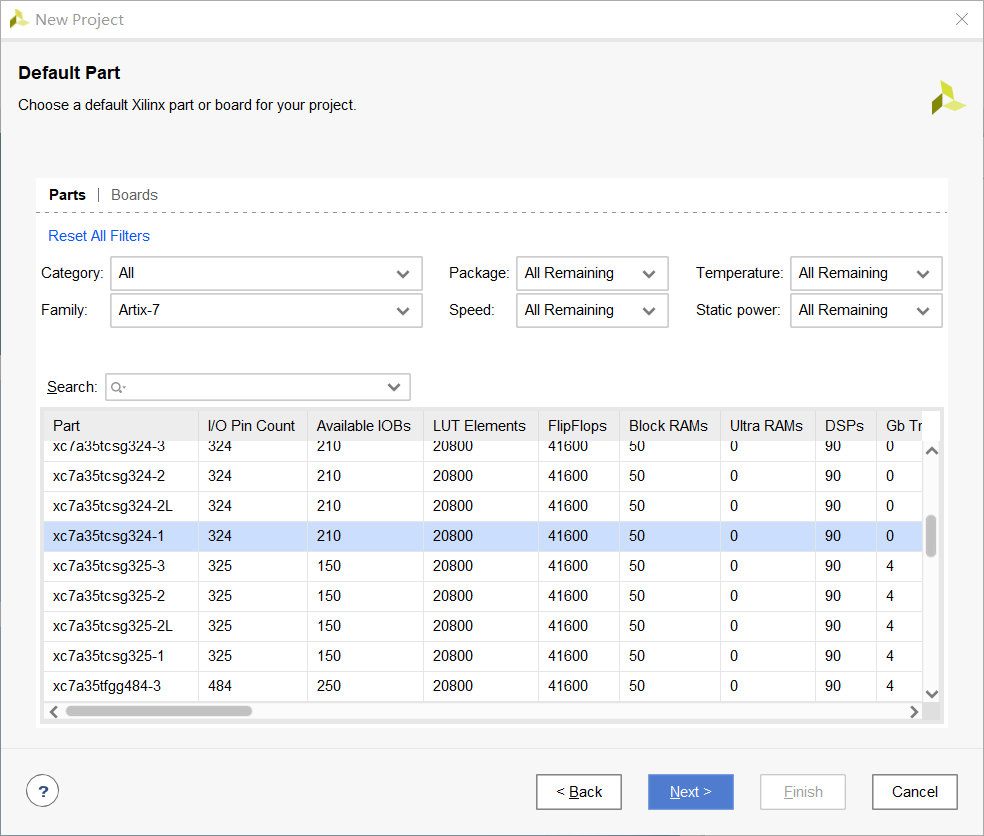
\includegraphics[width=.8\textwidth]{fig/Create4}
    \caption{选择板卡}
    \label{fig:Create4}
\end{figure}

当看到如图~\ref{fig:CreateDone}~所示界面后,说明项目创建完毕。

\begin{figure}[!htbp]
    \centering
    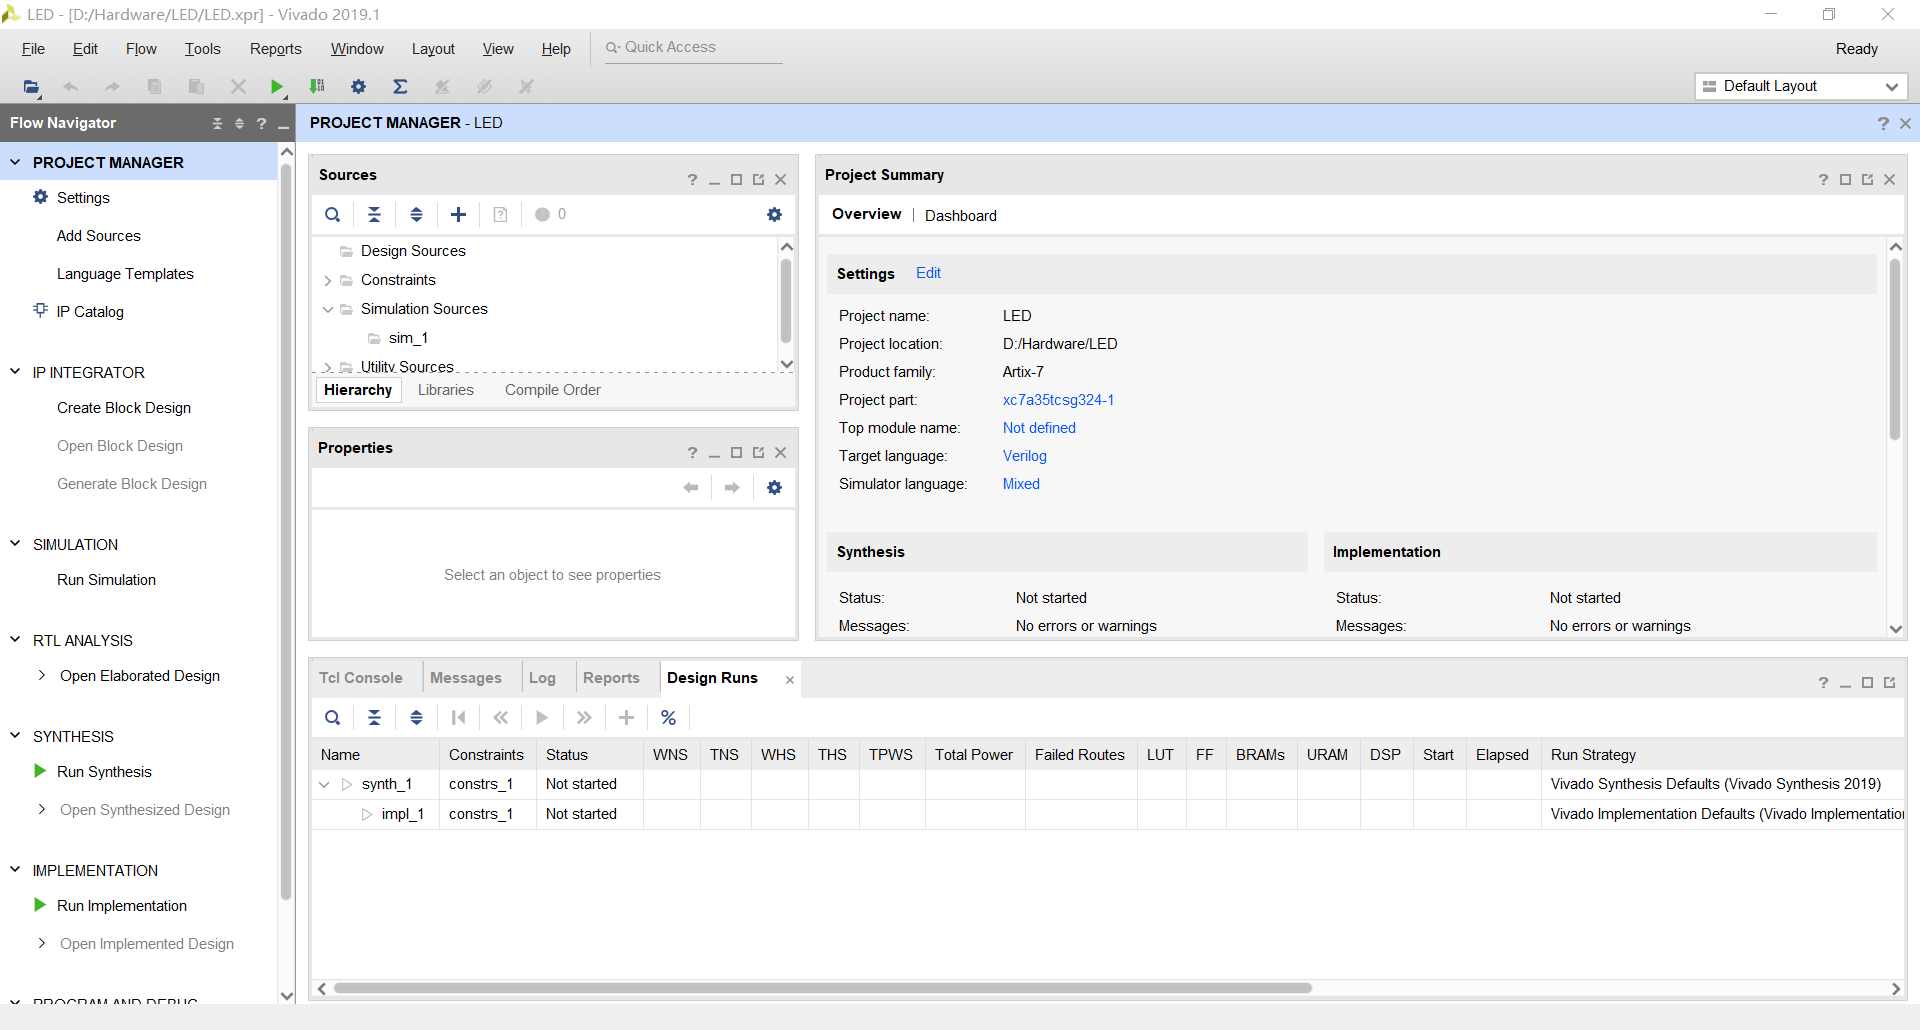
\includegraphics[width=.8\textwidth]{fig/CreateDone}
    \caption{Vivado 主界面}
    \label{fig:CreateDone}
\end{figure}

\newpage
\section{RTL 设计输入}

以使用 Verilog 完成 RTL 设计为例。Verilog 
代码都是以 “.v” 为后缀名的文件,可以在其他文件编辑器里写好,
再添加到新建的工程中,也可以在工程中新建一个再编辑。 
添加源文件,见图~\ref{fig:AddSource}~在 “Flow Navigator” 窗口下的 “Project Manager” 下点击
 “Add sources”,或者点击 “Source” 窗口下 “Add Sources” 按钮,
或者使用快捷键 “Alt + A”,到达图~\ref{fig:AddSource1}~所示界面。

\begin{figure}[!htbp]
    \centering
    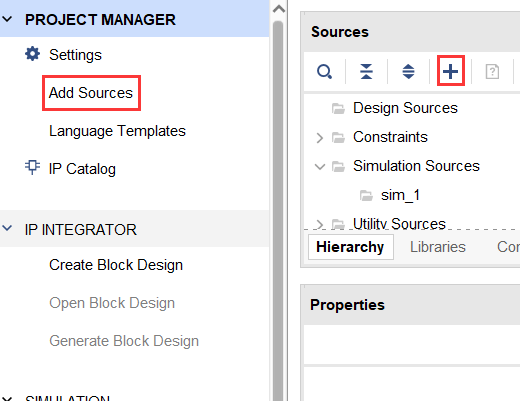
\includegraphics[width=.8\textwidth]{fig/AddSource}
    \caption{添加代码文件}
    \label{fig:AddSource}
\end{figure}

添加设计文件。选择 “Add or create design sources” 来添加或新建
 Verilog 或 VHDL 源文件,点击 “Next”,到达图~\ref{fig:AddSource2}~所示界面。
 
 \begin{figure}[!htbp]
    \centering
    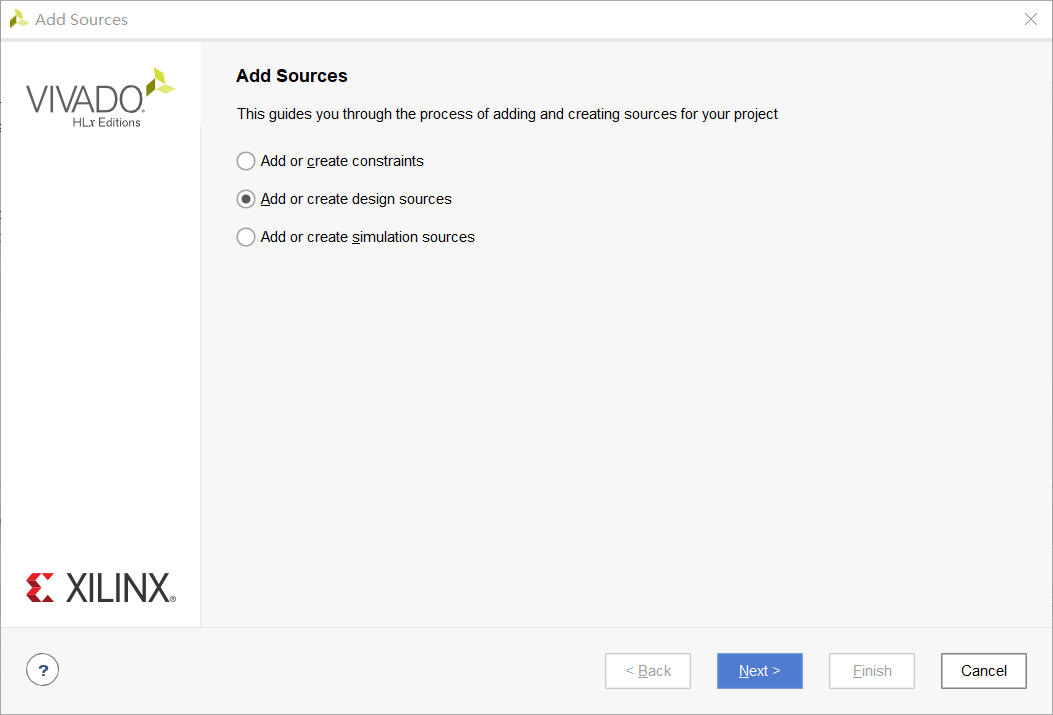
\includegraphics[width=.8\textwidth]{fig/AddSource1}
    \caption{选择文件类型}
    \label{fig:AddSource1}
\end{figure}

添加或者新建设计文件。如添加已有设计文件或者添加包含已有设计文件的文件夹,
选择 “Add Files” 或者 “Add Directories”,然后在文件浏览窗口选择已有
的设计文件完成添加。如创建新的设计文件,则选择 “Create File”。
这里新建文件。

\begin{figure}[!htbp]
    \centering
    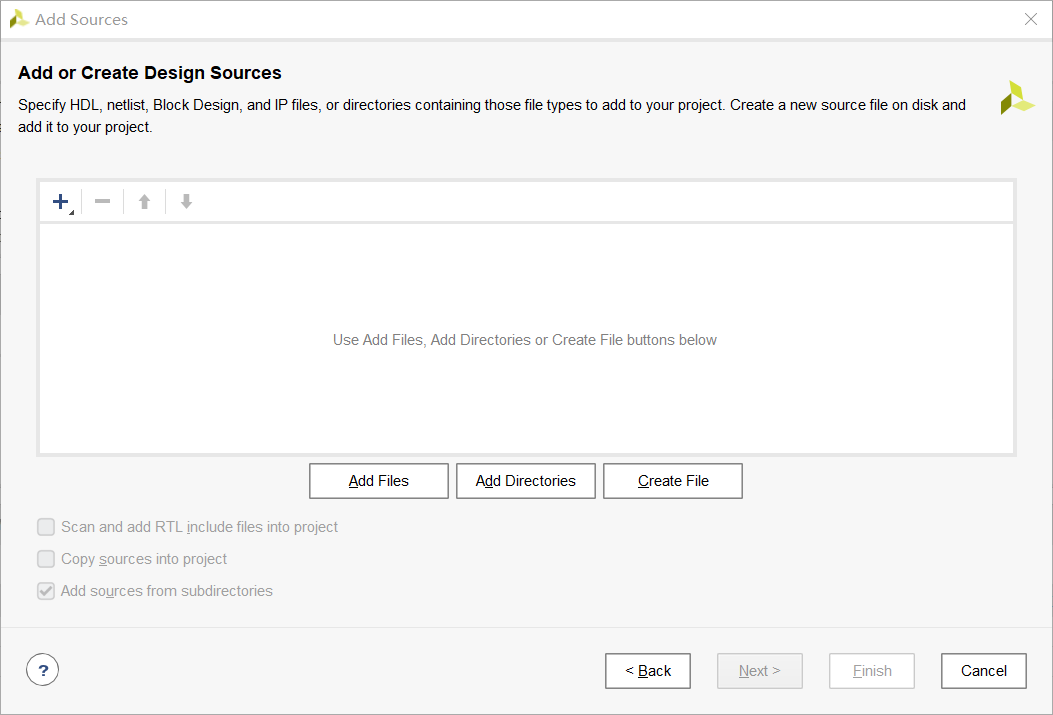
\includegraphics[width=.8\textwidth]{fig/AddSource2}
    \caption{添加文件}
    \label{fig:AddSource2}
\end{figure}

设置新创建文件的类型、名称和文件位置。

\begin{center}
    \begin{tikzpicture}
        \node [mybox] (box){%
            \begin{minipage}{0.9\textwidth}
                \qquad 文件名称和位置路径中不能出现中文和空格。 
            \end{minipage}
        };
        \node[fancytitle, right=10pt] at (box.north west) {注意};
    \end{tikzpicture}
\end{center}

继续添加设计文件或者修改已添加设计文件设置。添加完毕后点击 “Finish”,进入
模块端口设置。在 “Module Definition” 中的 “I/O Port Definitions”,
输入设计模块所需的端口,并设置端口 方向,如果端口为总线型,
勾选 “Bus” 选项,并通过 “MSB” 和 “LSB” 确定总线宽度。
完成后点击 “OK”。 端口设置也可以在编辑源文件时完成,
即可以在这一步直接点 “OK” 跳过。

设置完毕后,在 “Source” 窗口内可以看到新添加的文件。双击打开该文件,
即可输入代码。代码如下:

\begin{lstlisting}{language=Verilog}
`timescale 1ns / 1ps 

module flowing_light(
	input clk,
	input rst,
	output [15:0] led
);
 
    reg [23 : 0] cnt_reg;
	reg [15 : 0] light_reg; 
 
 
    always @ (posedge clk) begin
		if (!rst)
			cnt_reg <= 0;
		else
			cnt_reg <= cnt_reg + 1;
	end 
 
 
    always @ (posedge clk) begin
		if (!rst)
			light_reg <= 16'h0001;
		else if (cnt_reg == 24'hffffff) begin
			if (light_reg == 16'h8000)
				light_reg <= 16'h0001; 
            else
				light_reg <= light_reg << 1;
			end
		end
		
	assign led = light_reg;
	
endmodule
\end{lstlisting}

\begin{center}
    \begin{tikzpicture}
        \node [normalbox] (box){%
            \begin{minipage}{0.9\textwidth}
                \qquad 尽管 Vivado 的编辑器可以很好地提示错误的位置,但是
                其使用体验仍然不算是很好。为了更好的代码编写体验,建议使用
                Visual Studio Code 或者是 GNU Emacs 配合对应的插件进行
                RTL 代码的编写。然后将之导入 Vivado 进行仿真等后续操作。
            \end{minipage}
        };
        \node[normaltitle, right=10pt] at (box.north west) {建议};
    \end{tikzpicture}
\end{center}

\section{功能仿真}

Vivado 集成了内置的 Vivado Simulator,使用过 ModelSim 的同学可以
很快地掌握其使用方式。

首先添加测试激励文件。在 “Source” 中 “Simulation Sources” 右击选择
 “Add source”。之后通过和之前类似的方式添加测试激励文件,唯一需要注意的
 是要在第一个界面选择 “Add or Create Simulation Sources” 而不是
 “Add or Create Design Sources”。

在新建的测试激励文件内输入如下内容:

\begin{lstlisting}{language=Verilog}
`timescale 1ns/1ps
module flowing_light_tb(); 
 
reg clk; 
reg rst;

wire [3 : 0] led; 
 
flowing_light u0(
    .clk(clk),
    .rst(rst),
    .led(led)); 

parameter PERIOD = 10; 

always begin
    clk = 1'b0;
    #(PERIOD/2) clk = 1'b1;
    #(PERIOD/2);
end 
 
initial begin
    clk = 1'b0;
    rst = 1'b0;
    #100;
    rst = 1'b1;
    #100;
    rst = 1'b0;
    #100;
    rst = 1'b1;
end 
endmodule 
\end{lstlisting}

添加文件后,需要确认我们添加的激励文件是否是仿真的顶层文件,如果在 “Simulation Sources”
内我们的激励文件未被加粗,我们需要右击该文件并将之 “Set as Top”。确认无误后进入仿真。在左侧 
“Flow Navigator” 中点击 “Simulation” 下的 “Run Simulation” 选项,
并选择 “Run Behavioral Simulation” 一项,进入图~\ref{fig:Sim1}~所示的仿真界面。 

\begin{figure}[!htbp]
    \centering
    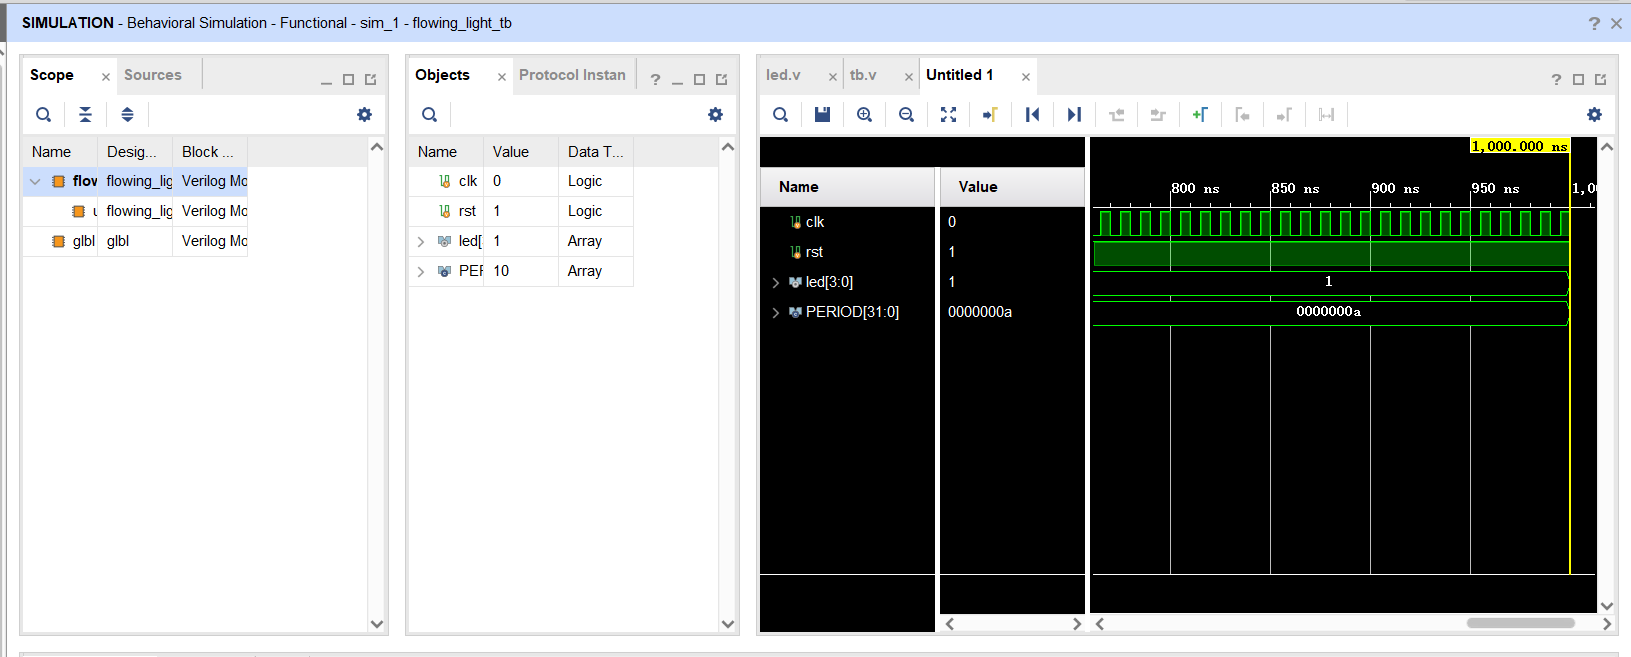
\includegraphics[width=1\textwidth]{fig/Sim1}
    \caption{仿真界面}
    \label{fig:Sim1}
\end{figure}

可通过左侧 “Scope” 一栏中的目录结构定位到想要查看的模块内部信号,
在 “Objects” 对应的信号名称上右击选择 “Add To Wave Window”,
将信号加入波形图中。仿真器默认显示 I/O 信号,由于这个示例不存在内
部信号,因此不需要添加观察信号。

可通过选择工具栏中的选项来进行波形的仿真时间控制。
如图\ref{fig:Sim2}所示工具条,分别是复位波形(即清空现有波形)、
运行仿真、运行特定时长的仿真、仿真时长设置、仿真时长单位、
单步运行、暂停、重启动。

\begin{figure}[!htbp]
    \centering
    
\includegraphics[width=0.8\textwidth]{fig/Sim2}
    \caption{仿真控制按钮}
    \label{fig:Sim2}
\end{figure}

在波形显示窗口上侧是如图\ref{fig:Sim3}所示的波形图控制工具,由左到右分别是:
查找、保存波 形配置、放大、缩小、缩放到全显示、
缩放到光标、转到时间 0、转到时间的最后、前一个跳变、
下一次跳变、添加标记、前标记、下一个标记、交换光标、设置。在信号上右击可以
调整进制数等信息。通过这些可以帮助我们观察仿真波形是否符合预期功能。

\begin{figure}[!htbp]
    \centering
    
\includegraphics[width=0.8\textwidth]{fig/Sim3}
    \caption{波形控制按钮}
    \label{fig:Sim3}
\end{figure}

在查看波形检查设计功能正确性后,我们就可以点击 “Synthesis” 下的 
“Run Synthesis” 开始后续操作。

\section{添加约束文件}

\subsection{引脚约束}
综合完成后,打开 “Open Synthesised Design”,在右上角的 “Layout” 处选择
“I/O Planning”。

\begin{figure}[!htbp]
    \centering
    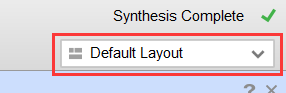
\includegraphics[width=0.5\textwidth]{fig/Con1}
    \caption{Layout}
    \label{fig:Con1}
\end{figure}

在界面右下方的选项卡中切换到 “I/O Ports” 一栏,
并在对应的信号后,在 “Site” 一列输入对应的 FPGA 管脚标号
(或将信号拖拽到右上方“Package”图中对应的管脚上),
并指定“I/O std”,在我们的 FPGA 中 “I/O Std” 应设置为 “LVCMOS33” ,
表明 I/O标准是 3.3V 的 LVCMOS。具体的 FPGA 约束管脚和 I/O 电平标准,
可参考对应板卡的原理图或提供的常用的引脚对应关系表。

完成约束后点击左上方工具栏中的保存按钮,提示添加新的约束文件使综合过时失效。
点击 “OK”。 新建 XDC 文件或选择工程中已有的 XDC 文件。
选择 “Create a new file”,输入 “File name”,
点击 “OK” 完成约束过程。 

直接编写 xdc 文件完成约束也是可以的,但是不在本文的讨论范围。

\section{时序约束}

添加时序约束的主要作用是使 Vivado 优化综合策略与布局布线,
以满足时序约束条件,同时也可以为时序分析提供参考依据。这一部分的详细叙述
不在介绍的范围内,请查阅 Vivado 的官方文档。

打开之前新建的 xdc 文件,在最后添加如下内容:

\begin{lstlisting}{language=tcl}
create_clock -period 8.000 -name clk_pin -waveform {0.000 4.000} [get_ports clk]
set_input_delay -clock [get_clocks *] 0.000 [get_ports rst]
set_input_delay -clock [get_clocks *] -min -0.500 [get_ports rst]
set_output_delay -clock [get_clocks *] 0.000 [get_ports -filter { NAME =~  "*" && DIRECTION == "OUT" }] 
\end{lstlisting}

如此就算是设置好了时钟,并定义了输入/输出的延迟。

\section{上板运行}

在 “Flow Navigator” 中点击 “Program and Debug” 下的 “Generate Bitstream” 
选项,工程会自动完成综合、 布局布线、Bit文件生成过程,完成之后,可点击 
“Open Implemented Design” 来查看工程实现结果。 

布线完成后,在比特流文件生成完成的窗口选择“Open Hardware Manager”,
进入硬件管理界面。连接 FPGA 开发板的电源线和与电脑的下载线,打开 FPGA 电源。点击上方
绿色横幅的 “Open Target” 下的 “Auto Connect” 即可连接设备。

\begin{center}
    \begin{tikzpicture}
        \node [normalbox] (box){%
            \begin{minipage}{0.9\textwidth}
                \qquad 初次连接 FPGA 时可能会出现 “\color{red}{ERROR: [Labtoolstcl 44-494] There is no active target available for server at localhost.
                Targets(s) ", jsn1" may be locked by another hw\_server.}” \color{black}{这样的错误。此时在任务管理器终止} \color{red}{\textbf{hw\_sever}} \color{black}{进程即可}。
                如果找不到设备/无法连接,首先确认 FPGA 端的 MicroUSB 接在了 JTAG 口上,如果还是
                不行,请更换电脑端的 USB 口重试。
            \end{minipage}
        };
        \node[normaltitle, right=10pt] at (box.north west) {提示};
    \end{tikzpicture}
\end{center}

\begin{figure}[!htbp]
    \centering
    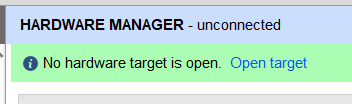
\includegraphics[width=0.5\textwidth]{fig/Hrd1}
    \caption{连接硬件}
    \label{fig:Hrd1}
\end{figure}

连接成功后,在目标芯片上右击,选择 “Program Device”。
在弹出的对话框中 “Bitstream File” 
一栏已经自动加载本工程生成的比特流文件,
点击 “Program” 对 FPGA 芯片进行编程。
 
\begin{center}
    \begin{tikzpicture}
        \node [normalbox] (box){%
            \begin{minipage}{0.9\textwidth}
                \qquad 如果没有自动加载文件的话,可以在 \textbf{<项目路径>/<项目名>.runs/impl\_1} 文件夹找到 bit 文件。
            \end{minipage}
        };
        \node[normaltitle, right=10pt] at (box.north west) {提示};
    \end{tikzpicture}
\end{center}

编程后即可在 FPGA 上观察实验结果。

\section{使用 ILA 在线调试}

\begin{center}
    \begin{tikzpicture}
        \node [mybox] (box){%
            \begin{minipage}{0.9\textwidth}
                \qquad 相对仿真调试,在线调试对调试思想和技巧有更高的要求,调试过程
                也更需要耐心以及毅力。在发现上板结果与预期不一致时,请先重点排查其他问题,最后再使用在线调试的方法,以
                节约时间。
            \end{minipage}
        };
        \node[fancytitle, right=10pt] at (box.north west) {注意};
    \end{tikzpicture}
\end{center}

Integrated Logic Analyzer (ILA) IP 核是一款逻辑分析器内核,
可用于监控设计中 的内部信号。ILA 内核包括现代逻辑分析器的大量高级特性,
如布尔触发器方程式以及边缘过渡触发器。由于 ILA 内核能够与正在监控的
设计保持同步,因此对设计应用的所有设计时钟限制也都会应用于 ILA 内核
中的组件。 

在 FPGA 开发过程中,我们可能会遇到仿真完全正常但是上板异常
的情况。此时就需要使用 ILA 来抓取需要查看的信号,并上板观察。 
下面我们依然以流水灯实验了解如何使用 Vivado 内置的 ILA 核。

\subsection{确定需要抓取的信号}

在 RTL 源码中,给想要抓取的信号添加 mark\_debug 信号即可。 
对于 SystemVerilog/Verilog 而言,
使用 (*mark\_debug = "true"*) 来设定需要抓取的信号。
\begin{lstlisting}
    input           branch_taken,
    input [31:0]    branch_address, 
 
(*mark_debug = "true"*) output logic [31:0]     pc_address
); 
 
    (*mark_debug = "true"*) logic [31:0] pc_address_next;
\end{lstlisting}
如果使用 VHDL 的话,使用如下所示方法设置需要抓取的信号: 
\begin{lstlisting}
    signal debug_wire : std_logic;
    attribute MARK_DEBUG : string; 
    -- Marks an internal wire for debug 
    attribute MARK_DEBUG of debug_wire : signal is “TRUE”; 
\end{lstlisting}

设置后,重新综合以更新网表文件。

\subsection{设置 DEBUG CORE}

在综合完成后,需建立调试核。点击工程左侧 SYNTHESIS -> Open 
Synthesized Desgin -> Set Up Debug(如图~\ref{fig:ILA1}~)。之后
会进入如图\ref{fig:ILA2}所示的界面。

\begin{figure}[!htbp]
    \centering
    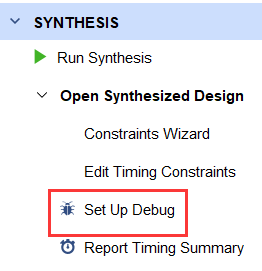
\includegraphics[width=0.3\textwidth]{fig/ILA1}
    \caption{设置 DEBUG CORE}
    \label{fig:ILA1}
\end{figure}

\begin{figure}[!htbp]
    \centering
    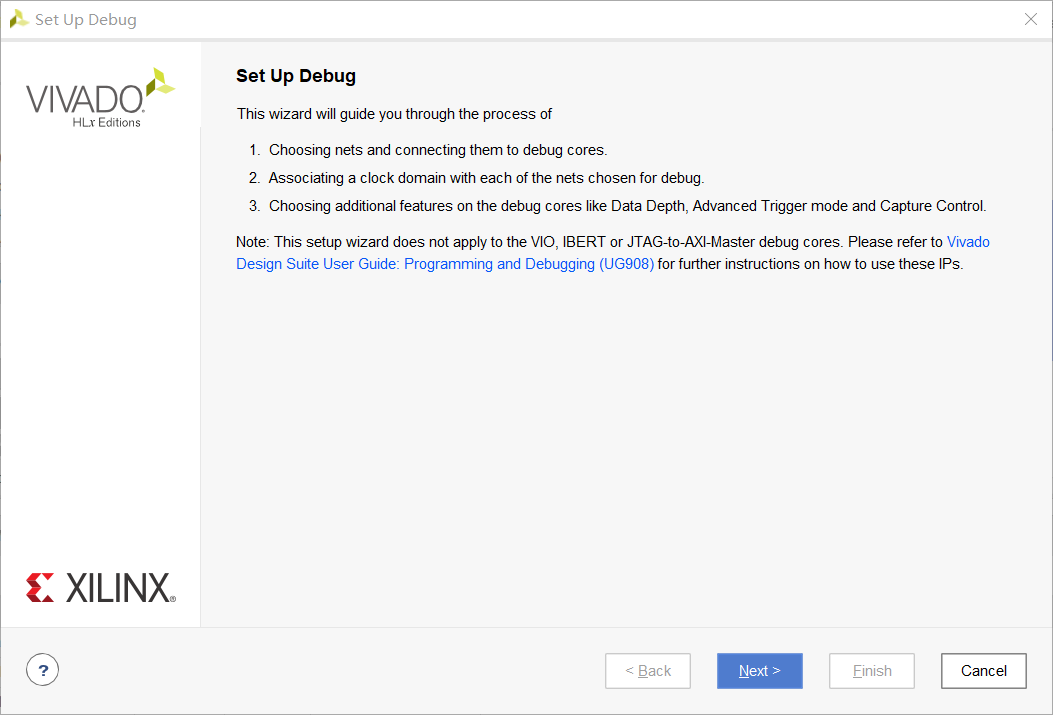
\includegraphics[width=0.8\textwidth]{fig/ILA2}
    \caption{设置 DEBUG CORE}
    \label{fig:ILA2}
\end{figure}

一路下一步,在下一个界面我们可以看到之前设置了 mark\_debug 属性的信号都被
列在了这里。我们也可以通过下方的 “Find Nets to Add…” 选项添加新的信号。选择好需要查看的信号后,
点击下一步,进入图片~\ref{fig:ILA3}~所示界面。 在这一界面内我们可以指定取样深度和一些高级设置,如果没有特殊需求的话,只需要选
中 “Capture Control” 选项即可。 
 之后进入下一步,点击完成。开始布局布线,生成比特流。最后使用 Hardware 
Manager 将生成的 .bit 文件烧入 FPGA 内,同时选中对应的 .ltx 文件以便 Vivado 收集数
据(这一步通常 Vivado 会自动选择 .bit 文件同名的 .ltx 文件)。 

\begin{center}
    \begin{tikzpicture}
        \node [normalbox] (box){%
            \begin{minipage}{0.9\textwidth}
                \qquad 通过 “Find Nets to Add…” 选项
                按钮添加新的信号时,要注意由于 Vivado 默认的综合策略会对设计进行跨边界优化,
                可能会出现需要查看的信号被更名/优化掉的情况。通过在项目设置中将 
                flatten\_hierarchy 开关选项设置为 none 可以避开这个问题。
            \end{minipage}
        };
        \node[normaltitle, right=10pt] at (box.north west) {提示};
    \end{tikzpicture}
\end{center}

\begin{figure}[!htbp]
    \centering
    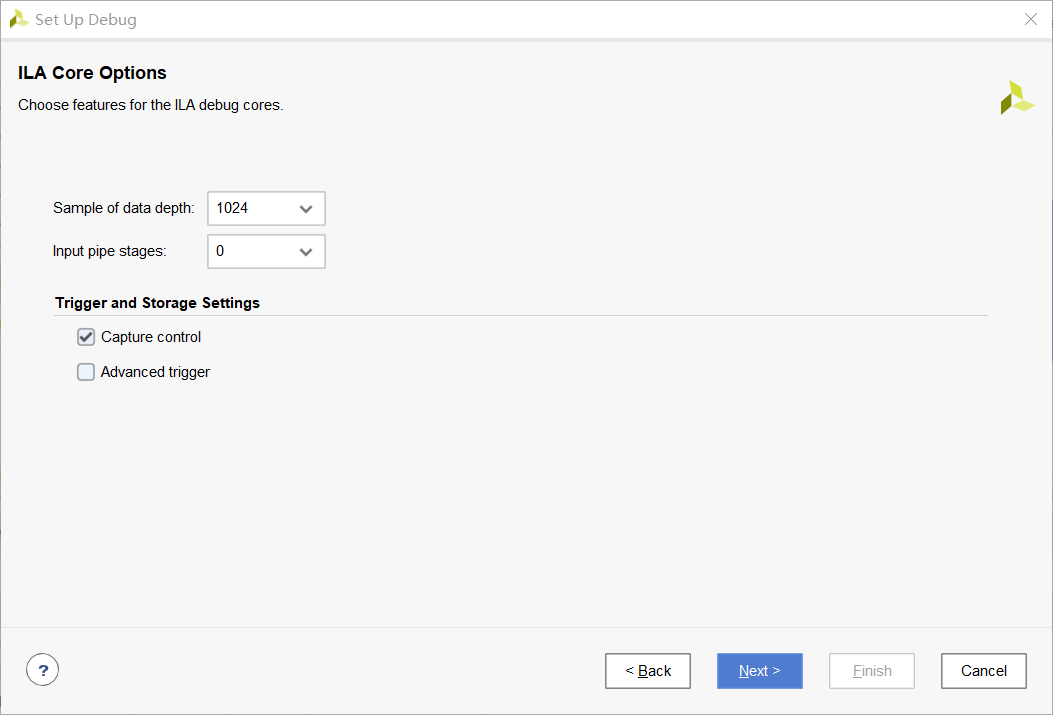
\includegraphics[width=0.8\textwidth]{fig/ILA3}
    \caption{设置 DEBUG CORE}
    \label{fig:ILA3}
\end{figure}

下载完成后,Hardware Manager 会变为如图~\ref{fig:ILA4}~所示界面。
窗口上方是类似仿真器的虚拟示波器,左下方是当前 ILA 的状态,右下方是
设置触发条件的窗口。

通过设置触发条件,我们可以抓取到特定状态下的信号信息。在左下方的窗口内点击
"+" 号,即可选择信号添加触发条件。Vivado 支持添加多个触发条件。

\begin{figure}[!htbp]
    \centering
    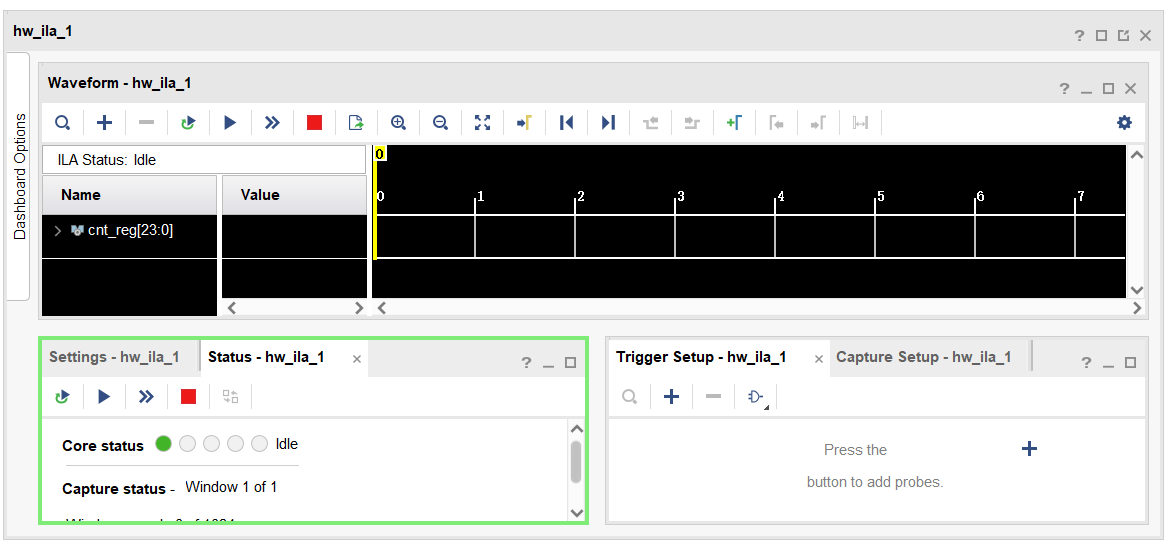
\includegraphics[width=0.95\textwidth]{fig/ILA4}
    \caption{ILA 调试窗口}
    \label{fig:ILA4}
\end{figure}

触发条件建立后,就可以启动波形抓取了,最关键的有三个触发按键,
即图~\ref{fig:ILA5}~ 圈出的3个按键:

\begin{itemize}
    \item 左起第一个,设定触发模式,有两个选项:单触发;循环触发。
    当该按键按下时,表示循环检测触发, 那么只要触发条件满足,
    波形窗口就会更新。当设置为单触发时,就是触发一次完成后,
    就不会再检测 触发条件了。
    比如,如果我们设定触发条件是 PC=0xbfc00690,那
    么如果该 PC 被多次执行到。如果设定 为单触发,
    那按下 FPGA 板上的复位键,波形窗口只会展示第一次触发时的情况。
    如果设定循环触发, 那么波形窗口会以 Refresh rate 
    不停刷新新捕获的触发条件。
    \item 左起第二个,等待触发条件被满足。点击该按键,就是等待除法条件被满足,展示出波形。 
    \item 左起第三个,立即触发。点击该按键,表示不管触发条件,立即抓取一段波形展示到窗口中。 
\end{itemize}

\begin{figure}[!htbp]
    \centering
    
\includegraphics[width=0.3\textwidth]{fig/ILA5}
    \caption{抓取按钮}
    \label{fig:ILA5}
\end{figure}

点击抓取后,抓取到的信号会显示在示波器内。其中如果设置了触发条件,符合触发条件的位置
会以红色实线标出,如图~\ref{fig:ILA6}~。

\begin{figure}[!htbp]
    \centering
    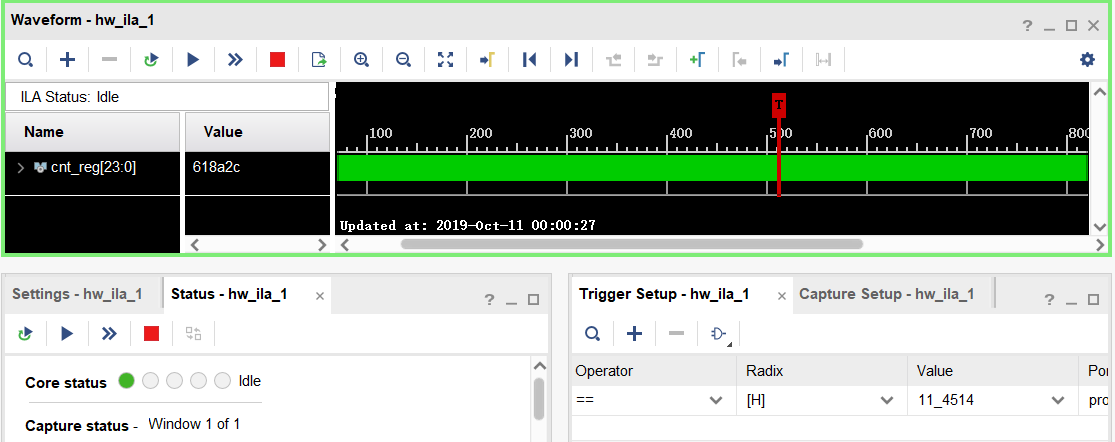
\includegraphics[width=0.95\textwidth]{fig/ILA6}
    \caption{抓取结果}
    \label{fig:ILA6}
\end{figure}

剩下的 debug 过程,就和仿真 debug 类似了,
去观察波形。但在线调试时,你无法直接添加之前未被添加 
debug mark的信号。在线调试过程中,可能需要不停的重新设置信号并综合布线,不停的更换触发条件,
不停的按复位键。 

对于需要保存下来数据的情况,我们可以使用 
Vivado 提供的
 tcl 指令 write\_hw\_ila\_data 实现,指令实例如下: 

\begin{lstlisting}
write_hw_ila_data -csv_file [get_property DIRECTORY [current_project]]/trace.csv [upload_hw_ila_data hw_ila_1]  
\end{lstlisting}

该指令会把示波器中显示的数据保存到项目目录下的 trace.csv 文件内。

\section{结语}
以上就是对 Vivado 开发流程的简单介绍。如果在实际开发中遇到了任何问题,请
善用搜索引擎以及 Vivado 提供的报错信息。

如果想要了解更多 Vivado 的使用方法,可以在 Xilinx 官网查找其使用指南。

\end{document}